\section{Future work}\label{sec:cutForTime}
As discussed in Section \ref{sec:shape_up}, the management approach Shape Up was used to plan and execute the tasks of this thesis. Because of this approach, also called \emph{fixed appetite, variable scope}, some ideas that were planned for the visualization dashboard were ultimately cut for time. These ideas could and should be considered if future work aims to further build on the prototype created for this thesis.

\subsubsection*{Show more detailed tooltips for both visualizations}\label{fw_tooltips}
The current implementation of the tooltips has two major drawbacks:
\begin{enumerate}
    \item They cannot be styled in any way---the style attribute only shows text that cannot be styled using CSS.
    \item The title attribute can only be used for visualizations which consist of several distinct HTML-elements, like the bar chart that was built using one div-container per day. More advanced visualizations without this clear mapping of one-element-per-day, like this prototype's visualization showing the development of the sentiment over time, cannot make use of the title attribute.
\end{enumerate}

Thus, future work should implement tooltips that do not rely on the title attribute. This would effectively solve the two problems mentioned above. The custom tooltip-element could be styled using standard CSS, and---if properly implemented---the tooltip can also be used for different visualization types. 

\subsubsection*{Showing trends in tooltips}
\begin{wrapfigure}{L}{0.3\textwidth}
    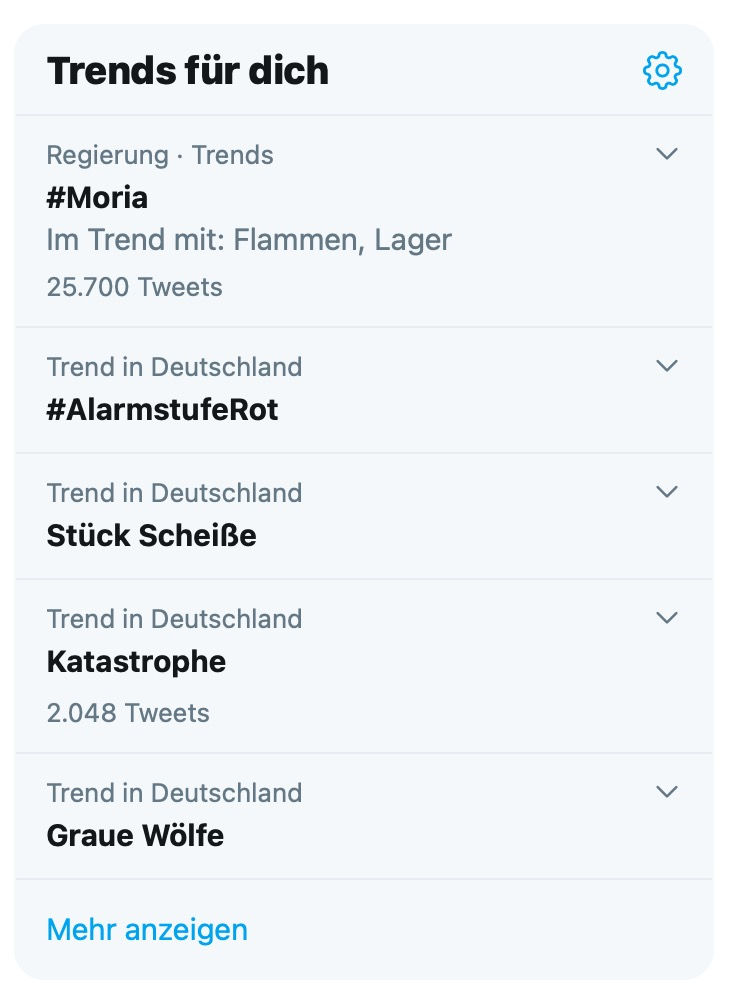
\includegraphics[width=0.28\textwidth]{images/twitter_trends.jpg}
    \caption{The trending topics on twitter. Collected on September 9th, 2020, 8.28 am}
    \label{fig:twitter_trends}
\end{wrapfigure}
One feature that was not sufficiently finished when the user tests started, and was thus left out completely, was a \emph{trend analysis} based on the collected tweets. The plan was to show users the trending topics for each day in the visualization. Due to Twitter's limitations in their API, it was not possible to retrieve the daily trends that Twitter already collects and shows.

To overcome this limitation, collocations were calculated for the tweet texts of each day. Collocations are \say{a lexical phenomenon} that \say{cover[s] word pairs and phrases that are commonly used in language} (\cite[2]{mckeown2000collocations}), which means that these are word pairs that encounter together more often than by pure chance. The idea was that by calculating collocations using the tweets of a day, those word pairs could be phrases that were talked about on this day. While for some days the results seemed promising, for most of the days the calculated word pairs did not give much information. Tweaks on the algorithm calculating the collocations could have yielded more informative results, but these tweaks could not be implemented before the user tests started.

Nevertheless, the user tests showed that participants wanted additional context for their findings to gain deeper knowledge from the visualizations. Showing the daily trends in the tooltip could satisfy this requirement without cluttering the interface too much.

\subsubsection*{Use more attributes from the tweet-objects}
As shown in chapter \ref{sec:fetchedData}, the country of origin for every tweet was collected. With this, a visualization could have shown differences in tweeting behavior between different countries. A theoretical example would be the question if tweets about a Covid-19 vaccine that come from Russia are more positive than tweets about a vaccine that were tweeted from other countries. As only around 20,000 out of the 2.5 million tweets that were collected contained the origin country, this feature was not implemented.

During tweet collection, some data attributes about the user who sent the tweet were collected, like their user name, their self-description, and their friend count. These attributes would have allowed performing some analysis on who sent which kinds of tweets – e.g., whether accounts with a lot of followers tend to send more positive or more negative tweets. These attributes were ultimately unused.

Another data point that was collected, but not used, was the verification status of the tweets' authors. The initial plan was to offer users an option to compare tweets from verified and unverified sources. The plan was to include a toggle that breaks up the existing bar chart and line chart with another dimension \emph{is\_verified}. This would have added a lot of complexity to the visualizations for the users. Because this work focuses on visualizations that can be easily read and understood by laymen, this feature was eventually scrapped before the user tests.

Using these additional data points could help users to generate further insight into the dataset. Collecting these data points is no additional work, as they are always contained in the tweet object that Twitter's API sends as a response to the endpoint.
